\documentclass{gd-llncs}
%\documentclass[preprint,3p,12pt]{elsarticle}

\usepackage{graphicx}
\usepackage[]{subfig}
\usepackage{svg}
\usepackage[]{pdfpages}
\usepackage[]{svg}

\graphicspath{{./images/}}
% \journal{Computational Geometry: Theory and Applications}

%\newtheorem{theorem}{Theorem}
%\newtheorem{problem}{Problem}
%\newtheorem{lemma}{Lemma}
%\newtheorem{proposition}{Proposition}
%\newenvironment{proof}{\noindent \emph{Proof}: }{\qed}

\newcommand{\comm}[1]{}
\newcommand{\TODO}[1]{{\color{magenta}{#1}}}
\newcommand{\new}[1]{\textcolor{green}{#1}}
%\newcommand{\note}[1]{\textcolor{blue}{[#1]}}

\newcommand{\df}[1]{\mbox{\textbf{#1}}}
\def\Cost{\text{\emph{routing cost}}}
\def\aCost{\text{\emph{additional cost}}}
\newcommand{\gv}{\widetilde{G}}
\newcommand{\ink}{I}
\newcommand{\cc}{C}
\newcommand{\inkcoeff}{k_{\textit{ink}}}
\newcommand{\lencoeff}{k_{\textit{len}}}
\newcommand{\capcoeff}{k_{\textit{cap}}}
\DeclareMathOperator{\nul}{\textit{null}}
\newcommand{\cdt}{$\mathcal{T}$}
\newcommand{\unpath}{$\mathcal{L}$}
\newcommand{\triset}{$\mathcal{U}$}
\newcommand{\plg}{$\mathcal{P}$}
\newcommand{\obst}{$\mathcal{O}$}
\begin{document}


\title{Browsing large graphs with MSAGLJS, a graph draph drawing tool in JavaScript }
\author{%
  Lev Nachmanson  \and
  Xiaoji Chen
}%
\institute{
  Microsoft Research, US,\\
  \email{levnach@hotmail.com, cxiaoji@gmail.com},\\
  Msagljs github home page:
  \texttt{https://github.com/microsoft/msagljs}
}
\maketitle
%\ead{levnach@microsoft.com}
%\address[LN]{Microsoft Research, USA}

%\ead{spupyrev@gmail.com}
%\address[SP]{Ural Federal University, Russia}

\begin{abstract}
  There has been progress in visualization of large graphs recently. Still, interacting with a large graph in the browser with the same ease as browsing an online map, inspecting the high level structure and zooming to the lower details, is still an unsolved problem, in our opinion. In this paper we describe MSAGLJS's approach to two aspects of this problem. Firstly, we give a novel algorithm for edge routing, where the edges do not overlap the nodes. The algorithm does not necesserely creates optimal paths but is efficient and creates visually appealing paths.

  Secondly, to facilitate graph vizualization with DeckGL, we propose a new simple and efficient approach to tiling. The approch guarantees that in every view the number of visible entities is not larger than a predefined bound.
\end{abstract}


\section*{Introduction}

\label{sec:intro}
\section*{Related work}
Links to large graph visualization


\cite{graphexp}

\cite{graphviz}

\cite{regraph}

\cite{skewed}

\cite{circos}

\cite{gibson2013survey}

machine learing approach
\cite{kwon2017would}

\cite{lin2013interactive}

\cite{cosmograph}

\section*{Edge routing}
The edge routing starts, as in~\cite{dwyer2010fast}, by building a spanner graph, an approximation of the full visibility graph. The spanner, see Fig.~\ref{fig:spanner}, is built on a variation of a Yao graph, which was introduced independently by Flinchbaugh and Jones~\cite{flinchbaugh1981strong}  and Yao~\cite{yao1982constructing}. A Yao graph is defined by the set of cones with the apices at the vertices. The cones have the same angle, usually in the form of $\frac{2\pi} {n}$, where $n$ is a natural number. This way the cones with the apex at a specific vertex partition the plane as illistrated in Fig.~\ref{fig:yao}. For each cone at most one edge is created connecting the cone apex with a vertex inside of the cone.

\begin{figure}[]
  \centering
  \begin{minipage}[b]{0.5\textwidth}
    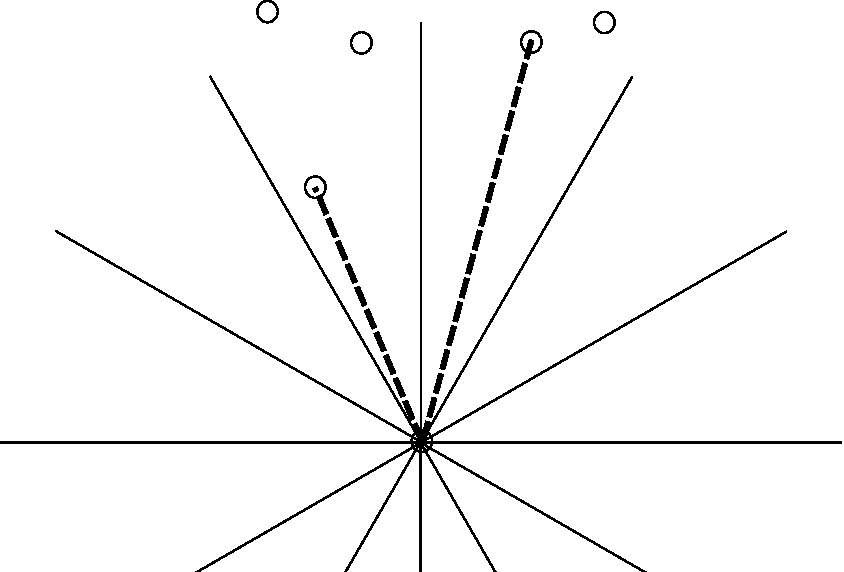
\includegraphics[width=\textwidth]{yao.pdf}
    \caption{\small{Yao graph}}
    \label{fig:yao}
  \end{minipage}

  \vfill
  \begin{minipage}[b]{\textwidth}
    \includesvg[width=\textwidth]{visibility_graph.svg}
    \caption{\small{Spanner graph is built using the idea of Yao graphs. The dashed curves are the original node boundaries. Each original curve is surrounded by a polygon with some offset to allow the polyline paths smoothing without intersecting the former. \\
      The edge marked by the circles is created because the top vertex is inside of the cone and it is the closest among such vertices to the cone apex. The apex of the cone is the lower vertex of the edge. \\MSAGLJS uses cone angle $\frac{\pi}{6}$, so the edges of the spanner can deviate from the optimal direction by this angle. Therefore the shortest paths on the spanner have length that is at most the optimal shortest length multiplied by $\frac{1}{\cos(\frac{\pi}.
        {6}}) \simeq 1.155$.}
    }
    \label{fig:spanner}
  \end{minipage}

\end{figure}


The approach of~\cite{dwyer2010fast} first builds a polyline path through the spanner, then applies some local modifications to shorten and smoothen the path. For shortening it tries to shortcut a vertex, as illustrated in Fig~\ref{fig:shortcut}. To smoothen it fits Bezier segments into the polyline corners, using the binary search to find the larger fitting segments,see Fig~\ref{fig:cornerfit}. While anylyzing performance of edge routing in MSAGLJS, we noticed that for a graph with more than 10000 edges these heuristics become the major bottleneck.
\begin{figure}[!tbp]
  \centering
  \begin{minipage}[b]{0.4\textwidth}
    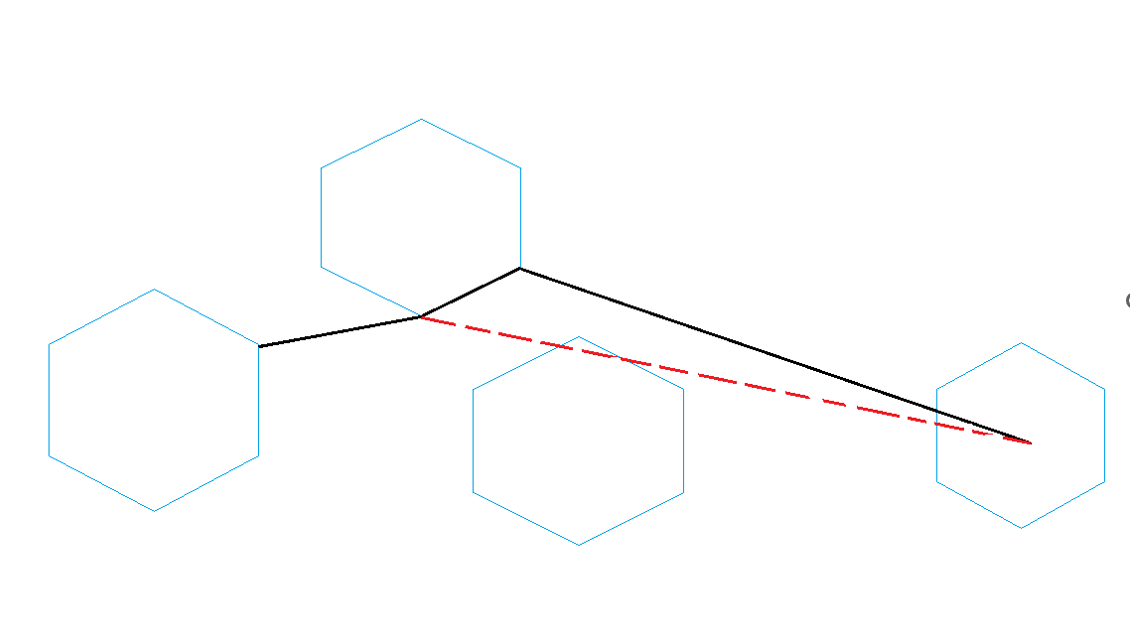
\includegraphics[width=\textwidth]{./naive_shorcut_now_working.png}
    \caption{Unsuccessful shortcut}
    \label{fig:shortcut}
  \end{minipage}
  \hfill
  \begin{minipage}[b]{0.4\textwidth}
    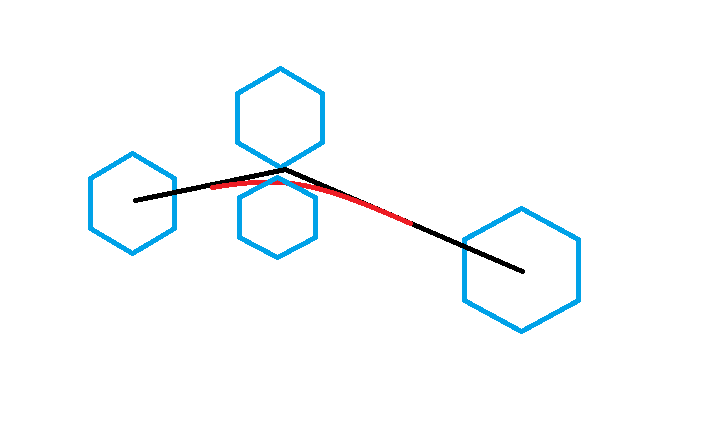
\includegraphics[width=\textwidth]{fillet_corner.png}
    \caption{Fitting a Bezier segment into a polyline corner}
    \label{fig:cornerfit}
  \end{minipage}

\end{figure}

The reason for this was that we queured if a curve intersects any node of the whole graph. In spite of optimizing these operations with R-Trees~\cite{guttman1984r}, about \%90 of the edge routing running time was spent on them. In addition, when the naive shortcutting of polyline corners fails the resulting path is not visually appealing, as shown in Fig.~\ref{fig:shortcut}.

We replace these heuristics with a more precize optimization.
\subsection*{Path optimization} {
The idea of using the path in a simple polygon optimization is not a new one. The authors of~\cite{dobkin1997implementing} used it, but only for hierarchical layouts, where a simple polygon, \plg, containing the path is available. They write: "If \plg~does not contain holes ... we can apply a standard “funnel” algorithm \cite{chazelle1982theorem,hershberger1994computing} for finding Euclidean shortest paths in a simple polygon". In general case, for a non-layered layout, they build the visibility graph which is very expensive.

Here we show how to build polygon \plg, and create a better path for any layout. Let us describe our method.

We call obstacles $\mathcal{O}$~the set of polygons covering the original nodes, see Fig.~\ref{fig:spanner}. Before routing edges we calculate a Constrained Delaunay Triangulation~\cite{delaunay1934sphere} on $\mathcal{O}$ and call it $\mathcal{T}$. Then for each edge of the graph we proceed with the following steps.

We route a path on the spanner, as illistrated by Fig.~\ref{fig:non_opt_path_L}. Let us call this path \unpath.


\begin{figure}[!tbp]
  \centering
  \begin{minipage}[b]{0.45\textwidth}
    \includesvg[width=\textwidth]{non_optimized_path_on_global_cdt.svg}
    \caption{Path \unpath~with \cdt, a fragment.}
    \label{fig:non_opt_path_L}
  \end{minipage}
  \hfill
  \begin{minipage}[b]{0.45\textwidth}
    \includesvg[width=\textwidth]{poly2.svg}
    \caption{Polygon \plg~containing \unpath.}
    \label{fig:polygon_with_path}
  \end{minipage}
  \vfill
  \begin{minipage}[b]{0.45\textwidth}
    \includesvg[width=\textwidth]{poly3.svg}
    \caption{New triangulation of \plg.}
    \label{fig:new_triangulation}
  \end{minipage}
  \hfill
  \begin{minipage}[b]{0.45\textwidth}
    \includesvg[width=\textwidth]{poly4.svg}
    \caption{Optimized path.}
    \label{fig:optimized_path}
  \end{minipage}
\end{figure}
Let $\mathcal{S}$ be the obstacle containing \unpath's start point, and $\mathcal{E}$ be the obstacle containing \unpath's end point.
To obtain \plg, let us consider \triset~, the set of all triangles ${t} \in \mathcal{T}$ such that
either ${t} \subset \mathcal{S} \cup \mathcal{E}$, or $t$ intersects \unpath~ and is not inside of any obstacle.
The union of \triset~gives us \plg. The boundary of \plg~comprizes all edges $e$ of the triangles from \triset~ such that $e$ is adjacent to exactly one triangle from \triset, see Fig.~\ref{fig:polygon_with_path}. \\
To apply the funnel algorithm~\cite{chazelle1982theorem,hershberger1994computing}, we need to have a triangulation of \plg~ such that every edge of the triangulation is either a boundary edge of \plg, or a diagonal of \plg. In our situation \triset~ usually does not have this property. We create a new Constrained Delaunay Triangulation of \plg, where the set of constrained edges is the boundary of \plg, see Fig.~\ref{fig:new_triangulation}.\\
Finally, we apply the funnel algorithm to obtain the path which is the shortest in the homotopy class of \unpath, see Fig.~\ref{fig:optimized_path}.\\

\begin{figure}[]
  \centering
  \includegraphics*[]{sleeve_diagonals_not_optimal.pdf}
  \caption{\plg~is not simple polygon. The dotted path is shorter than the dashed one, that was found be the routing.}
  \label{fig:non_optimal_path}
\end{figure}


The polygon \plg~is not neccesserely simple, as shown in Fig.~\ref{fig:non_optimal_path}.
In this example the path that we calculate with the funnel algorithm is not the shortest path inside of \plg.
\subsection*{Performance and quality comparison}
In Fig.~\ref{fig:improved_routing} we compare the paths generated by the old and the new method. We can see that the paths on the right fragment of the picture have no kinks. We also know that they are shorter. Arguably, the new method produces better paths.
\begin{figure}[]
  \centering
  \includegraphics*[width=0.5\textwidth]{comparison.png}
  \caption{The difference in quality between the old and the new edge routing. The arrows point to the kinks that were removed by the new method.}
  \label{fig:improved_routing}
\end{figure}

% new results\\
% % % driver.ts:172 loading graph gameofthrones.json with 407 nodes, and 2639 edges
% % % driver.ts:197 layout: 700.746826171875 ms
% % % driver.ts:203 routing: 1291.155029296875 ms
% % % \\
% % % loading graph b100.gv with 1463 nodes, and 5806 edges
% % % driver.ts:197 layout: 4445.96484375 ms
% % % driver.ts:203 routing: 5785.367919921875 ms
% \\
% loading graph composers.json with 3405 nodes, and 13832 edges
% driver.ts:197 layout: 1435.905029296875 ms
% driver.ts:203 routing: 20060.42578125 ms
% \\
% loading graph p2p-Gnutella04.JSON with 10876 nodes, and 39994 edges
% driver.ts:197 layout: 8258.957275390625 ms
% driver.ts:203 routing: 315084.2478027344 m\\
% --------------------------\\
% old results
% loading graph gameofthrones.json with 407 nodes, and 2639 edges
% driver.ts:197 layout: 746.14013671875 ms
% driver.ts:203 routing: 1001.654052734375 ms
% \\
% loading graph b100.gv with 1463 nodes, and 5806 edges
% driver.ts:197 layout: 4286.7490234375 ms
% driver.ts:203 routing: 5607.820068359375 ms
% \\
% \\
% loading graph composers.json with 3405 nodes, and 13832 edges
% driver.ts:197 layout: 1744.442138671875 ms
% driver.ts:203 routing: 510510.5849609375 ms
% \\
% loading graph p2p-Gnutella04.JSON with 10876 nodes, and 39994 edges
% driver.ts:197 layout: 7869.53076171875 ms
% driver.ts:203 routing: 375416.2248535156 ms
% new loading graph facebook_combined.txt with 4039 nodes, and 88234 edges
% driver.ts:172
% layout: 3192.4921875 ms
% driver.ts:197
% routing: 119058.66088867188 ms
% old loading graph facebook_combined.txt with 4039 nodes, and 88234 edges
% driver.ts:172
% layout: 3207.157958984375 ms
% driver.ts:197
% routing: 132194.51196289062 ms

% new loading graph lastfm_asia_edges.csv with 7626 nodes, and 27807 edges
% driver.ts:197 layout: 4256.56982421875 ms
% driver.ts:203 routing: 41438.64208984375 ms

% old loading graph lastfm_asia_edges.csv with 7626 nodes, and 27807 edges
% driver.ts:172
% layout: 4343.10498046875 ms
% driver.ts:197
% routing: 43277.473876953125 ms

% new loading graph deezer_europe_edges.csv with 28283 nodes, and 92753 edges
% driver.ts:197 layout: 30625.172119140625 ms
% driver.ts:203 routing: 1209277.4853515625 ms
%  old loading graph deezer_europe_edges.csv with 28283 nodes, and 92753 edges
%  driver.ts:197 layout: 20907.59521484375 ms
% driver.ts:203 routing: 1606911.0739746094 ms
%new loading graph b103.gv with 944 nodes, and 2438 edges
% driver.ts:197 layout: 1678.364990234375 ms
% driver.ts:203 routing: 2005.841796875 ms

% oading graph b103.gv with 944 nodes, and 2438 edges
%driver.ts:197 layout: 1652.553955078125 ms
%driver.ts:203 routing: 1628.798095703125 ms

% new loading graph ca-HepPh.txt with 12008 nodes, and 237010 edges
% driver.ts:197 layout: 12165.052001953125 ms
% driver.ts:203 routing: 494965.1198730469 ms
% old loading graph ca-HepPh.txt with 12008 nodes, and 237010 edges
% driver.ts:197 layout: 10407.01513671875 ms
% driver.ts:203 routing: 521223.0046386719 ms

Our experiments are summarized in Table.~\ref{tab:perf}. We see that the older approach outperforms the new one on the smaller graphs; those with the number of nodes under 2000. The new method is faster on the rest of the graphs. We still prefer to use the new method independently of the graph size since the total slowdown in insignificant, under a half second in our experiments, but the quality of the paths is better. On the larger graphs the new method runs faster and produces better paths, so it is an obvious choice.
\begin{table}
  \begin{center}
    \begin{tabular}{||c |c| c| c| c||}
      \hline
      graph name            & nodes & edges  & old method's time & new time \\ [0.5ex]
      \hline\hline
      social network        & 407   & 2639   & 1.0               & 1.4      \\
      \hline
      b103                  & 944   & 2438   & 1.6               & 2.0      \\
      \hline
      b100                  & 1463  & 5806   & 5.6               & 5.785    \\
      \hline
      composers             & 3405  & 13832  & 510.5             & 17.5     \\
      \hline
      p2p-Gnutella04        & 10876 & 39994  & 375.4             & 293.8    \\
      \hline
      facebook\_combined    & 4039  & 88234  & 132.2             & 119.1    \\
      \hline
      lastfm\_asia\_edges   & 7626  & 27807  & 43.3              & 41.4     \\
      \hline
      deezer\_europe\_edges & 28283 & 92753  & 1596.9            & 1209.3   \\
      \hline
      ca-HepPh              & 12008 & 237010 & 521.2             & 495.0    \\
      \hline
      % driver.ts:197 layout: 12165.052001953125 ms
      % driver.ts:203 routing: 494965.1198730469 ms
      % old loading graph ca-HepPh.txt with 12008 nodes, and 237010 edges
      % driver.ts:197 layout: 10407.01513671875 ms
      % driver.ts:203 routing: 521223.0046386719 ms
    \end{tabular}
    \caption{Performance comparison. The time is in seconds.}
    \label{tab:perf}
  \end{center}

\end{table}
\comm{
  \section{Further Examples}
}
\bibliography{main}
\bibliographystyle{ieeetr}
\end{document}
